% Header: Here are all packages used and some additional definitions
%%%%%%%%%%%%%%%%%%%%%%%%%%%%%%%%%%%%%%%%%%%%%%%%%%%%%%%%%%%%%%%%%%%

\documentclass[11pt,a4paper]{scrartcl}
\usepackage[margin=2.5cm]{geometry}
\usepackage[onehalfspacing]{setspace}
\usepackage{graphicx} % zum Einbinden von Graphiken
\usepackage[breaklinks=true,colorlinks=true,linkcolor=blue,urlcolor=blue,citecolor=blue]{hyperref} % für Links
\usepackage{amsmath,amsthm,amssymb} % Mathematik Umgebung 
\usepackage{icomma} % Intelligentes Komma, das den richtigen Abstand zwischen Dezimalzahlen als auch in Formeln wählt.
\usepackage{babel} % Deutsche Bezeichnungen bei Inhaltsangabe etc
\usepackage[T1]{fontenc}    % andere Schriftsatzkodierung für richtige Silbentrennung bei Umlauten
\usepackage[locale = DE,space-before-unit=true,per-mode = symbol]{siunitx} % Bessere Einheiten
\usepackage{booktabs,multirow} % Pakete zur Erstellung von Tabellen
\usepackage{placeins} % Definiert den Befehl “\FloatBarrier”, der die Ausgabe der davor eingebundenen Bilder erzwingt, befor der Text weiter geht. (Mit vorsicht zu verwenden)
%\usepackage[natbib,abbreviate=true,doi=false,style=numeric-comp,giveninits=true,sorting=none]{biblatex}
\usepackage{natbib} % Modernes Paket zur Erzeugung von Bibliografien (benötigt biber!)
\usepackage{bibentry}
\usepackage{csquotes} % Fortgeschrittene Funktionen für Zitate, für die deutsche Form der Anführungszeichen bei Referenzen
% Ort der .bib Datei, die die Datenbank für Literatur/Referenzen enthält.

\graphicspath{{Bilder/}}

\DeclareSIUnit{\dBm}{dBm}
\DeclareSIUnit[per-mode=reciprocal]\WN{\per\centi\meter}

%%%%%%%%%%%%%%%%%%%%%%%%%%%%%%%%%%%%%%%%%%%%%%%%%%%%%%%%%%%%%%%%%%%
\begin{document}
%
\titlehead{}
\onecolumn

\begin{center}
\textbf{\fontsize{14}{\baselineskip}\selectfont Deggendorf Institute of Technology}

\bigskip

\textbf{\fontsize{14}{\baselineskip}\selectfont Case study - Cyber-physical Production Systems using AM}

\bigskip

\textbf{\fontsize{12}{\baselineskip}\selectfont Under the guidance of }

\bigskip

\textbf{\fontsize{14}{\baselineskip}\selectfont Prof. Dr. Ing. Stefan Scherbarth}

\bigskip
\bigskip
\bigskip

\textbf{\fontsize{20}{\baselineskip}\selectfont Centrifugal Pump with Semi-open Single Vane impeller}

\bigskip

\bigskip

\bigskip

\textit{\textbf{\fontsize{14}{\baselineskip}\selectfont by}}

\bigskip

\bigskip

\bigskip

\textbf{\fontsize{14}{\baselineskip}\selectfont Group name: Vane Vortex\\ }
\bigskip
\textbf{\fontsize{14}{\baselineskip}\selectfont Group no:11\\ }
\bigskip
\bigskip
\textbf{\fontsize{14}{\baselineskip}\selectfont Thushar Tom, Matriculation No: 22202815\\ }
\textbf{\fontsize{14}{\baselineskip}\selectfont \\ }
\textbf{\fontsize{14}{\baselineskip}\selectfont Sreehari Giridharan, Matriculation No: 22200251 \\}
\textbf{\fontsize{14}{\baselineskip}\selectfont \\ }
\textbf{\fontsize{14}{\baselineskip}\selectfont Alla Durga Nooka Venkatesh, Matriculation No: 22207330 \\}
\textbf{\fontsize{14}{\baselineskip}\selectfont \\ }
\textbf{\fontsize{14}{\baselineskip}\selectfont Tran Hoang Duy Nguyen, Matriculation No: 22203230 \\}

\bigskip

\bigskip

\bigskip

Course period - March 2023 - July 2023\\



\bigskip

\bigskip


{\today}
\end{center}
\bigskip
\clearpage
%
%
\tableofcontents
\newpage

\listoffigures
\thispagestyle{empty}
\cleardoublepage
\pagenumbering{arabic} 
\newpage
%
%
\section{Abstract}
Zentrifugalpumpen mit halboffenen und einflügeligen Laufrädern sind vielseitig einsetzbar und werden in vielen Pumpenszenarien verwendet, z. B. in der Abwasserbehandlung, in der Industrie und in der Landwirtschaft. Sie werden typischerweise in Anwendungen eingesetzt, bei denen kleine Feststoffe, wie z. B. Erde und Schutt, die in der mit mittlerem Durchfluss fließenden Flüssigkeit suspendiert sind, gefördert werden müssen. Diese Pumpen sind bekannt für ihre zuverlässige Leistung, ihren hohen Wirkungsgrad, ihre gute Verstopfungsresistenz, ihre Wartungs-freundlichkeit und ihre Fähigkeit, mit verschiedenen Arten von viskosen und abrasiven Flüssigkeiten zu arbeiten. In diesem Bericht stellen wir das grundlegende Funktionsprinzip von Kreiselpumpen vor und unterscheiden die Laufradtypen nach ihren geometrischen Formen und Anwendungen, wobei wir uns besonders auf Kreiselpumpen mit halboffenen und einflügeligen Konstruktionen konzentrieren. Wir versuchen, einen Überblick über die Betriebsbedingungen, Leistungsparameter und Gleichungen zu geben, die den geometrischen Entwurf der erforderlichen Laufradkonfiguration bestimmen. Wir haben auch unseren Ansatz für den Entwurf und die parametrische Modellierung der Pumpe vorgestellt, wobei die beiden Hauptkomponenten das Laufrad und die das Laufrad umgebende Spirale sind, und zwar mithilfe eines Lua-Skripts in IceSL. Wir haben die Konzepte und ihre mathematischen Gleichungen, die zum Verständnis unseres Ansatzes erforderlich sind, näher erläutert. Der Inhalt unseres Lehrvideos wurde ebenfalls in diesem Bericht erläutert. Wir haben auch die Anwendungen, Vor- und Nachteile sowie die Zukunftsaussichten einer Kreiselpumpe mit einem halboffenen und einflügeligen Laufrad diskutiert.\\

Centrifugal pumps with semi-open and single vane impellers are versatile and widely used in a lot of pumping scenarios like sewage and wastewater treatment, industries, and agriculture. They are typically used in applications which require the passage of small solid materials, such as soil and debris, suspended in the fluid flowing at a medium flow rate. These pumps are known for their reliable performance, high efficiency, good resistance to clogging, ease of maintenance, and ability to work with different kinds of viscous and abrasive fluids. In this report, we present the fundamental working principle of centrifugal pumps and discern the types of impeller according to their geometric designs and applications, while giving the particular focus on centrifugal pumps with semi-open and single vane design configurations. We try to give an overview of the working conditions, performance parameters and equations which determine the geometric design of the required impeller configuration. We have also presented our approach to designing and parametrically modeling the pump, with two main components being the impeller and the volute surrounding the impeller, using Lua script in IceSL. We have elaborated on the concepts and their mathematical equations required to understand our approach. The contents of our educational video have also been outlined in this report. We have also discussed the applications, advantages, disadvantages as well as future prospects of a centrifugal pump with a semi-open and single vane impeller.

\section{Introduction}
Pumping is the process of imparting energy to a fluid and thus moving it from one point to another or raising it to the required height. The applications that involve pumping liquids have been universal, finding their use in various industries, housing, agriculture, wastewater treatment, and even the human body for that matter. There are various kinds of pumps,  which should be chosen considering  the application scenario and its specific requirements. When choosing a pump, parameters such as capacity range of the liquid flow, required differential head, Net Positive Suction Head Available (NPSHA), pump rotary speed, shape of the head capacity curve, characteristics of the working liquid, determine the kind of pump that needs to be used \cite{lobanoff}.

\subsection{Centrifugal pumps in general}
Centrifugal pumps are one of the oldest pumps to exist and are still extensively used in various applications. The fundamental components of a centrifugal pump are an impeller and a casing or volute around it. The impeller is connected to a shaft at its center or eye, and is normally powered by a motor. The impeller has certain structures called vanes on it, fitted into shroud plates in different configurations.\par

The impeller is usually immersed in the liquid that needs to be pumped, which is collected through the inlet of the pump. When the impeller is rotated, with the help of the vanes, it also causes the surrounding liquid to rotate, imparting the centrifugal force to the particles of the fluid, pushing the fluid radially outwards immediately into walls of the volute and then to the pump outlet. 

\begin{figure}[h]
    \centering
    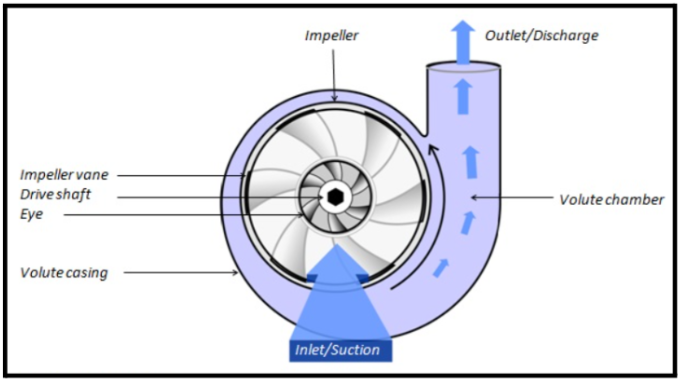
\includegraphics[scale=0.8]{image1.png}
    \caption{ Fundamental units of a centrifugal pump - impeller and casing [1]}
    \label{fig:image1}
\end{figure}
Thus, the rotational mechanical energy is transferred to the fluid, thereby increasing the kinetic energy of the fluid. The progressively increasing shape of the volute accumulates fluid at the discharge end, consequently increasing the static pressure. Meanwhile, at the suction end, this displacement of fluid causes negative pressure and consequently, draws in more fluid into the impeller and continues the process. \par

In the initial condition, when there is no liquid present in the pump, the negative pressure caused by the rotation of the air is not strong enough to draw the fluid into the impeller. Hence, the centrifugal pumps should be filled with fluid in the beginning and this process is called the “Priming”.\par 

Centrifugal pumps come in different configurations, and it is essential to choose an optimal design configuration that is well-suited for the specific task or application.

\subsection{Impeller design and casing}
\subsubsection{Comparing Closed, open and semi-open impeller designs}
When an impeller is enclosed by shroud plates on both sides, this is referred to as a "closed" impeller design. These are typically employed in applications involving clear liquids, but they are not suitable for pumping liquids that contain suspended solid materials. Since it has mechanical shroud plates on both ends of the impeller, it can withstand higher pressure and flow rates. However, when a fluid with suspended solids is pumped through this design, the risk of clogging is very high. Closed impeller designs are usually preffered when the application demands pumping hot or cryogenic liquids.\par

“Open” impeller design refers to the design where the vanes are attached to a center hub that is directly mounted on the shaft. As there are no shroud plates on either side of the impeller. Hence, this design configuration allows the passage of suspended solid materials in the liquid. However, since the impeller doesn’t have shroud plates on either side, the mechanical strength of the design is low and thus cannot withstand higher pressures and flow rates of the fluid.\par

“Semi-open” impeller design refers to the design where the impeller has a shroud plate on one side of the impeller, and this helps in giving the impeller design sufficient mechanical strength to withstand higher pressure and flow rates, and the ability to pass the solids suspended in the fluid. Semi-open impeller designs also offer better efficiency as the disk friction from the front plate is eliminated [7].

\begin{figure}[h]
    \centering
    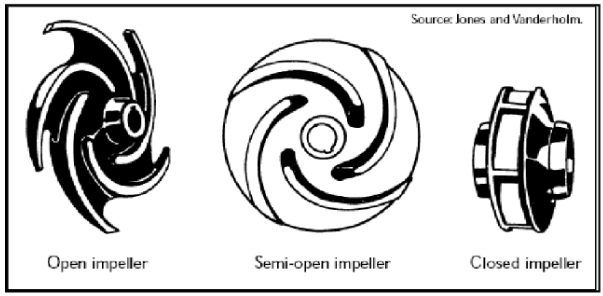
\includegraphics[scale=0.8]{image2.png}
    \caption{open, semi-open and closed impeller designs [3]}
   
    \label{fig:image2}
    
\end{figure}
\subsubsection{Vane Quantity (No. of Vanes)}
The number of vanes in an impeller design is one of the key factors that has to be selected based on the application. A higher number of vanes can result in an increase in the head at a given speed and improved efficiency. However, with more number of vanes, the space between the vanes is limited, which increases the risk of clogging suspended solid materials in the fluid. In a single vane impeller, the impeller passage is large, thereby reducing the risk of clogging. Vane quantity is also responsible for quantities such as radial thrust. Multi-vane impellers, which are usually symmetrical, can only give limited radial thrust. On the other hand, single-vane impellers offer an improved radial thrust and thus offer better support in building up the static pressure of the fluid at the exit end. 
\subsubsection{ Casing - Volute}
Volute is the curved structure around the impeller that is designed to navigate the flow of the fluid out of the impeller. It helps in the conversion of kinetic energy of the fluid to the static pressure and thus collecting the fluid and routing it to the discharge nozzle. The volute has an increasing cross-sectional area in the direction of the flow of the liquid. This progressively increasing area along the flow direction will help to accommodate newly added liquid and also to reduce the exit flow velocity. The reduction in exit flow velocity results in the increase of the static pressure that is being developed, which is required to overcome the resistance of the pumping system.

\subsection{Scope of the report: Centrifugal pumps with semi-open and single vane impellers }
In this report, we focus on the “Centrifugal pump with semi-open and single vane impeller” configuration. This design configuration is best suited for the applications that require “Anti-clogging” properties since the single vane and shroud plate on one side of the impeller allows the passage of small suspended materials in the liquids, while providing the impeller sufficient mechanical strength to withstand higher flow rates and viscosities. These features make semi-open single vane impellers suitable for applications such as sewage pumping, wastewater treatment, and chemical processing.  

\begin{figure}[h]
    \centering
    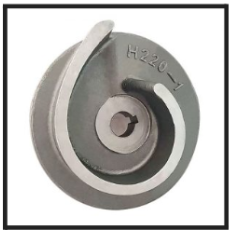
\includegraphics[scale=0.8]{image3.png}
    \caption{Semi-open and single vane impeller [2]}
   
    \label{fig:image3}
   
\end{figure}
In this report, we analyze the design of the state-of-the-art centrifugal pump with a semi-open and single vane impeller and understand the parameters that decide the geometry of the machine element. Later, we will present an interesting geometric approach using Bézier curves to design the impeller. The equations and the approach used in the report are the basis for parametric modeling of the machine element that make use of Lua scripting in IceSL. These can be used in additive manufacturing of the machine element. We discuss the advantages and disadvantages of semi-open and single vane impellers over other types of impellers. The scope of this report is limited to the geometric parameters discussed in this article without getting into the performance metrics that affect the design of our impeller. This report also clarifies the scope of the information that is being used in the educational video and provides references to the educational material that can be covered in order to get a deeper understanding of the subject material.

\section{Geometry of the machine elements}
\subsection{State-of-the-art design of the machine elements}
\begin{figure}[h]
    \centering
    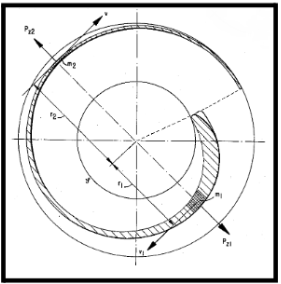
\includegraphics[scale=0.8]{image4.png}
    \caption{Semi-open and single vane impeller [4]}
    
    \label{fig:image4}
    
\end{figure}

In this section, we present the general procedure that is followed when designing a centrifugal pump with a semi-open and single vane impeller. The geometric design of the impeller depends on various parameters and their relationships with one another. 

The impeller design varies according to the requirements specifications required by the task at hand. Initially the task at the hand is analyzed and design flow rate Q, total head H, and rotation speed n are determined. From these design specifications, the specific speed $n_s$  can be obtained. The value of specific speed  $n_s$ is used to determine the target pump efficiency $\sigma$ using past records. The past records are used to estimate volumetric efficiency $\sigma_v$ and mechanical efficiency $\sigma_m$ and from these values the theoretical head $H_{th}$ for finite number of blades can be determined by the following equation:    
$$ H_{th}=\frac{\eta_v\eta_mH}{\eta}\hspace{1cm}(1)$$
Now, the appropriate blade outer diameter $D_2$ needs to be calculated. The outlet circumferential velocity constant $K_{u2}$ is one of the most important factors to determine the performance of the pump. However, as pointed out by Toyokura[3], the $K_{u2}$ values of the analogous pumps vary according to size of the pumps as the total head H changes depending on pump efficiency. Hence, the modified design method uses specific speed $n_{sth}$ determined using the following equation in which $H_{th}$ is used instead of H :
$$n_{sth}=\frac{n(60Q)^{1/2}}{H_{th}^{3/4}}\hspace{1cm}(2)$$
The blade outlet diameter $D_2$ can be determined using the following equation:
$$D_2=\frac{60K_{\mu_2}\sqrt{2gH_{th}}}{{\pi}n}\hspace{1cm}(3)$$
The semi-open single vane configuration only allows only solid materials of certain dimensions through them. When the size of the solid particles suspended in the fluid, particle size d is specified, the blade outlet width b2 can be observed to be in a range satisfying the relation: $b_2$ , is greater than or equal to d. The number of blades z should be less in number if a large particle is expected to go through the impellers. The single vane design configuration is usually preferred when a large particle size is specified. 

The blade outlet meridian velocity $v_{m2}$  considering the flow channel area reduction rate can be determined by the following equation where $\sigma_2$ denotes the circumferential blade thickness at the blade outlet:
$$v_{m2}=\frac{Q}{\eta_v({\pi}D_{2}-z\sigma_2)b_2}\hspace{1cm}(4)$$
In the next step, the blade outlet angle $\beta_{2b}$ is assumed. Wiesner’s formula[7] is used to estimate the slip factor k. For determining the slip factor k, the blade inlet diameter $D_1$ is assumed and the relative velocity at the blade outlet $w_2$ when we finite number of blades are considered is given by the equation:
$$w_2=\sqrt{V^2_{m2}+\left[ku_2+\frac{v_{m2}}{tan\;\beta_{2b}}\right]^2}\hspace{1cm}(5)$$
According to Stepanoff, the ratio of relative velocities at the inlet and the outlet of the blade $w_2/w$ is 0.8 to 0.87[2]. 

 The blade inlet meridian velocity $v_{m1}$ considering the flow channel area reduction rate can be determined by the following equation:
$$V_{m1}=\frac{Q}{\eta_v({\pi}D_1-2\sigma_1)b_1}\hspace{1cm}(6)$$
$\sigma_1$ denotes the circumferential blade thickness at the blade inlet, $b_1$ denotes the blade inlet width. 
\paragraph{}

In this design configuration, we can observe a sharp decrease in velocity of the fluid which is coming in from the suction inlet, near the blade inlet when the fluid suddenly changes its direction from axial to radial generating an uneven flow. It is determined that excessive reduction in the velocity of fluid can result in poor efficiency. Hence, we should also include calculations regarding suction velocity in the design of the impeller. Hence, $V_{m1}/V_0$ is also included as a design parameter.
\paragraph{}
The suction diameter $D_0$ can be determined by the following equation:
$$D_0=\sqrt{\frac{4Q}{\eta_v{\pi}v_0}}\hspace{1cm}(7)$$
The blade inlet angle is determined the following equation:
$$\beta_{1b}=sin^-1\left[\frac{v_{m1}}{w_1}\right]\hspace{1cm}(8)$$
Assuming that there is no prewhirl, the blade inner diameter can be determined by the equation:
$$D_1=\frac{60v_{m1}}{{\pi}n\;tan\;\beta_{1b}}\hspace{1cm}(9)$$
The blade inlet width can thus be determined using the following equation:
$$b_1=\frac{Q}{\eta_v({\pi}D_1-z\sigma_1)v_{m1}}\hspace{1cm}(10)$$
WIth the above calculation of the parameters, all the important values that determine the design of the impeller are calculated. 
\paragraph{}
The net positive suction head Hsv can be determined by the following equation:
$$H_{sv}=\lambda_1\;\frac{w^2_{1}}{2g}+\lambda_2\;\frac{v^2_1}{2g}\hspace{1cm}(11)$$
$\lambda_1$ and $\lambda_2$ denote the experimental coefficients of velocity heads and this equation can be used to check for the possibility of cavitation. Now, various simulations and convergence studies are made to fix the values of the parameters calculated to support the semi-open and single vane design for the applications.
\subsection{Design considerations for volute:}
There are some general design considerations that need to be made in designing the volute. The objective of the volute is to convert the kinetic energy of the fluid into pressure. The casing of the pump has nothing to do with the head and hence it only deals with minimizing losses. In general, a single volute casing where there is only a single spiral shaped chamber around the impeller is the most preferred for a semi-open and single vane impeller since its design already incorporates some recirculation and backflow to balance the forces on the hydraulic impeller. If the pump is being designed to handle high viscous fluids at low flow rates, a double or even higher volute casings might be a better choice[10].
There are various methods to design the volute around the impeller. The design method according to Stepanoff[11] is based on the principle of kinetic energy.\par 
According to Stepanoff [11]
$$R=\frac{1}{2}\sqrt{\frac{{\theta}Q}{90^\circ{\pi}c_{\theta}}}\hspace{1cm}(12)$$
Where $\eta$ is the design angle from 0^$\circ$. to 360^$\circ$, Q is the flow rate, $c_υ$ is the specified velocity of the fluid. \par

There are many other equations that relate radius and design angle. But, the best method is only decided after we do extensive testing of the pump for best efficiency. One such other equation that relates radius and design angle proposed by Pfleiderer [10] is:

$$R=\frac{{\theta}Q}{720^\circ{\pi}c_{u,i}r_i}+\sqrt{\frac{{\theta}Q}{360^\circ{\pi}c_{u,i}}}\hspace{1cm}(13)$$
\\
\begin{figure}[h]
    \centering
    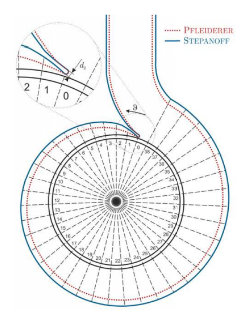
\includegraphics[scale=0.8]{image5.png}
    \caption{Comparison of design volute [10]}
    \label{fig:image4}
    
\end{figure}
\\

The inner radius of the volute is just a geometric relation with respect to other parameters like radius of the shroud. The sharp edge of the volute tongue that intersects with the impeller blades is called the cutwater. It has been determined experimentally that if the cutwater is less than 10\% of the outer radius of the impeller, it doesn’t affect the efficiency. But, if the cut water is between 10 to 20\%, the efficiency of the pump reduces by 1\% [6]. The space between the shroud and the outer volute casing at the cutwater is called clearance and is necessary to prevent contact between the casing and the rotating impeller. The clearance in the volute design must be carefully optimized to give the best pump efficiency which is determined by the best efficiency point (BEP) on the H-Q curve [11].   

\subsection{Construction method employed to design the machine element}
In this section, we present the ideas and concepts we have employed to design a centrifugal pump with a semi-open and single vane impeller. Usually, as discussed in section 3.1, the geometric values of the parameters that affect the design of the pump are calculated from the pump requirement specifications, since every requirement needs a respective design that best suits it. The method that we generated the impeller design is mostly geometric making use of various concepts.
\subsubsection{ Impeller}
One possible method to build the geometry of the impeller blade is to use the Bézier curve. Bézier curve is a curve built on a set of control points $P_0$ through $P_n$, where n is called the order of the curve (n = 1 for linear, 2 for quadratic, 3 for cubic, etc.). The first and last control points are the endpoints of the curve; meanwhile, the intermediate control points act like the guide for the curvature [4].\par
In this report, the proposed vane design calculation is done using the Bézier curve with 4 control points, means the order of curve(n) is 3 (cubic Bézier curve). The usage of Bézier curve in impeller design is efficient due to certain specific advantages.\par
Firstly, the Bézier curve offers the possibility to create a smooth curve based on its control points. Meanwhile, because the impeller shroud is a full circle shape, the impeller blade centerline could be mathematically simplified as a function of curvature radius over the wrap angle in polar coordinates. When combining these two things together, the Bézier curve becomes a convenient tool to generate an approximate function, which ensures the smooth transition of curvature radius throughout the wrap angle of the blade.\par
Secondly, the Bézier curve also provides the flexibility to adjust the middle part of the curve, while fixing the first and the last control points. This means, the starting and ending points of the impeller blade, which is directly calculated from inlet angle, outlet angle, and wrap angle of pump design, could be chosen first. After that, the curve connecting these 2 points could be created and modified with high flexibility.\par
The general mathematic equation of Bézier curve with 4 control points is developed as below [4]:
$$B(t)=(1-t)^3P_0+3(1-t)^2t\;P1+3(1-t)t^2P_2+t^3P_3$$
with 0<= t <= 1 and $P_0, P_1, P_2, P_3$ are the coordinates of 4 control points, B(t) is the function of the Bézier curve.\par

To make it easier for this particular use case, the 4 control points are declared by:\par

 - [$P_0$ P_3$]: Coordinates of P0 (starting point) and P3 (ending point)\par
 - $W_1$: distance between $P_0$ and $P_1$\par
 - $\alpha_1$: Relative angle that depicts the direction of $P_0$ heading 
   towards $P_1$\par
  -$W_2$: distance between $P_3$ and $P_2$ \par
- $\alpha_2$: Relative angle that depicts the direction of P3 heading towards $P_2$\par
The parameters $W_{1/2}$ and $\alpha_{1/2}$ give the convenience in controlling the Bézier curve, as it is directly related to how drastically the curve heads out from P0 to P1 and approaches the end from P2 to P3. The conversion from $W_{1/2}$ and $\alpha_{1/2}$ back to coordinates of $P_1$ and $P_2$ could be done easily by applying basic sin and cosin function:
\par

$$P_1(x)=P_0(x)+w_1cos(\alpha_1)$$
$$P_1(y)=P_0(y)+w_1sin(\alpha_1)$$
$$P_2(x)=P_3(x)-w_2cos(\alpha_2)$$
$$P_2(y)=P_3(y)+w_2sin(\alpha_2)$$

\begin{figure}[h]
    \centering
    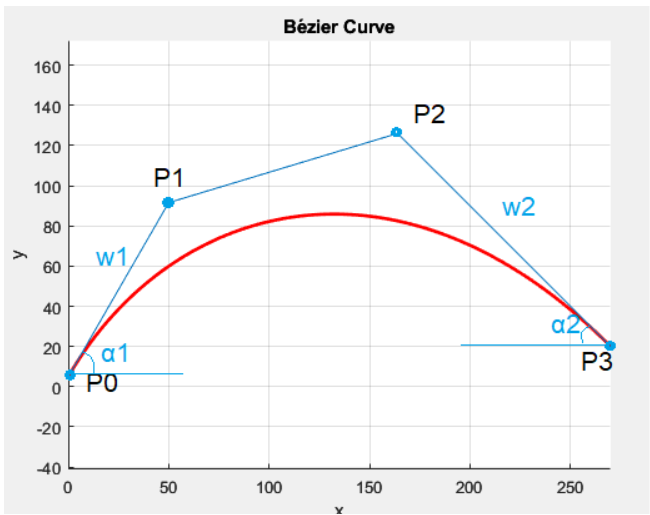
\includegraphics[scale=0.8]{image6.png}
    \caption{Fixing the control points of the Bézier curve using weights and angles}
    \label{fig:image4}
    
\end{figure}
\newpage
If we choose the coordinate of this Bézier curve as the angle displacement θ and curvature radius R of the blade element, where the blade element is a differential element on the blade geometry looping through the wrap angle, we will have a curve function describing the geometry of the blade in polar coordinate.


\begin{figure}[h]
    \centering
    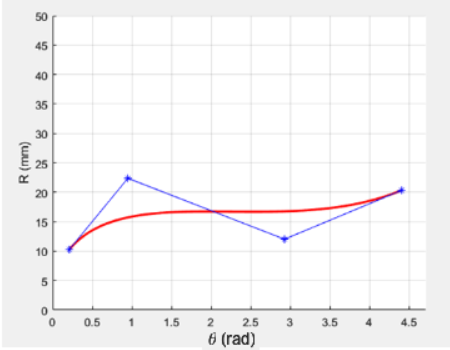
\includegraphics[scale=1]{image7.png}
    \caption{Radius parameter modeled in relation to the wrap angle 
}
    \label{fig:image4}
    
\end{figure}

Then, from the function of the Bézier curve above, the final geometry centerline could be easily displayed in polar coordinates.
\newpage


\begin{figure}[h]
    \centering
    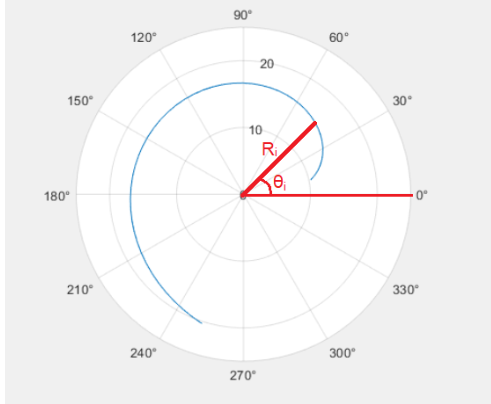
\includegraphics[scale=1]{image8.png}
    \caption{ Design of the blade centerline on the shroud in matlab }
    \label{fig:image4}
    
\end{figure}

To add the thickness to the blade, one simple method is to expand a constant thickness along the centerline. This method is simple to calculate but does not give the flexibility to optimize the blade in terms of material efficiency. Another possible method is to make the blade thickness vary so that there could be more material at the weak points of the blade and less material where fluid force is not critical. Again, Bézier curve could be applied here to give a smooth continuity of the thickness.
\begin{figure}[h]
    \centering
    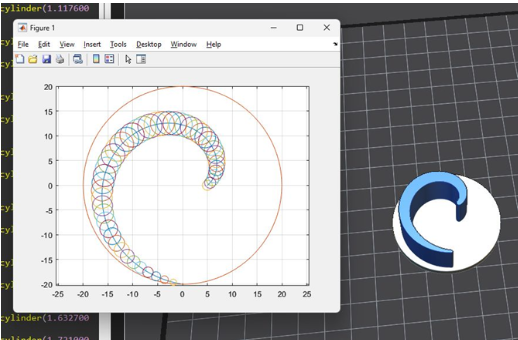
\includegraphics[scale=1]{image9.png}
    \caption{ Method employed to add thickness to the blade centerline using Bézier curve }
    \label{fig:image4}
    
\end{figure}

\subsubsection{Volute/ Casing: }
We propose a parametrized geometric method to design the outer casing around the impeller. User-defined clearance, inlet radius, outlet radius and casing thickness are being assumed as parameters.  We have chosen a logarithmic curve to define the change in outer diameter of the volute. And this control curve using inner and outer radius as extremes of the volute, encloses the impeller shape. Logarithmic curve is only one of the possible solutions as normally the outer shape of the volute is experimentally designed and tailored depending on applications.  
\begin{figure}[h]
    \centering
    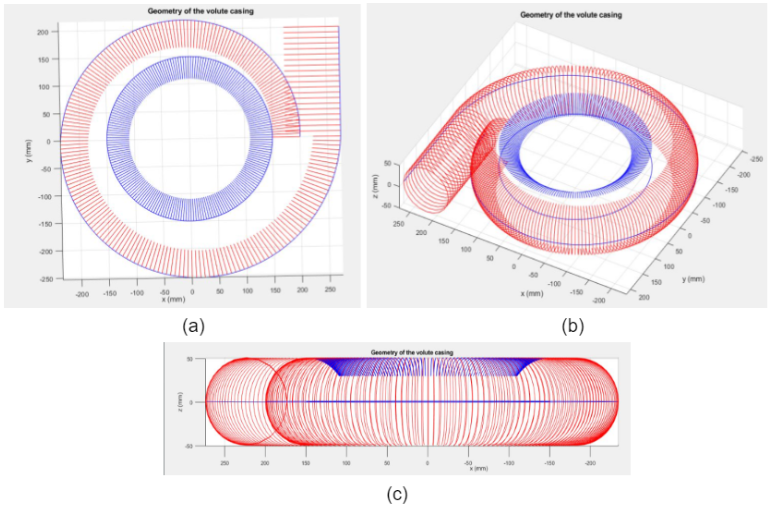
\includegraphics[scale=1]{image10.png}
    \caption{  a) Geometry of the volute casing in X-Y plane (b) Geometry of the volute casing in 3D view (c) geometry of the volute casing in X-Z plane
 }
    \label{fig:image4}
    
\end{figure}
\subsubsection{Nomenclature and scopes of the geometric parameters used:}
Most of the parameters are constrained to a working range by which they are bounded to generate the desired shape and structure. For instance, the user-defined outlet diameter is constrained by the space between the casing and the impeller, so that the blade of the impeller doesn't collide with the casing. We plan to take these relations between the parameters into account while working in the Lua script in IceSl. 

\begin{figure}[h]
    \centering
    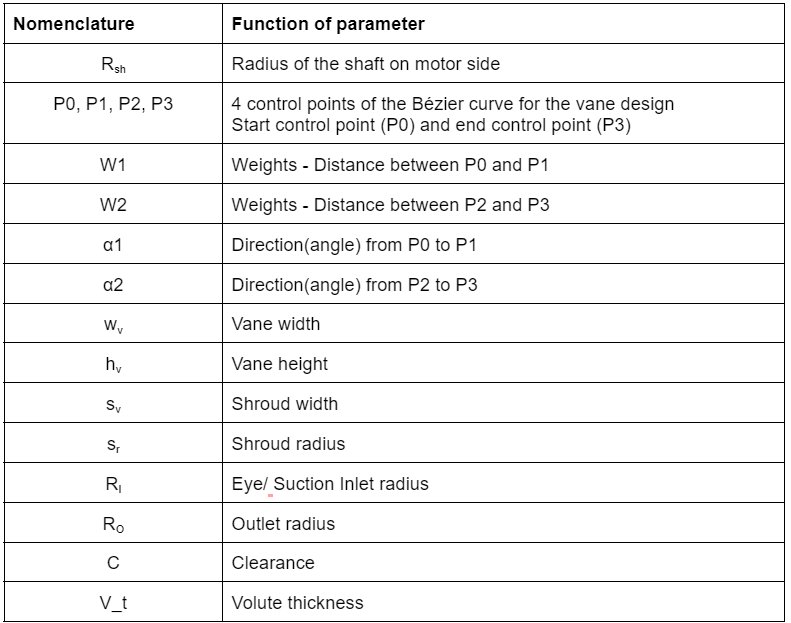
\includegraphics[scale=1]{image11.png}
    \caption{ Nomenclature of geometric parameters
 }
    \label{fig:image4}
    
\end{figure}
\newpage
\section{Advantages, Disadvantages and Alternative solutions}
\subsection{Advantages}
Using a centrifugal pump with a semi-open and single vane impeller comes with a lot of advantages.
\begin{enumerate}
        \item \textbf{Improved solids handling capability:} The semi-open design and larger passage area of the impeller enable it to efficiently pass small solid materials like sand or dirt that may be suspended in the liquid or slurry without experiencing clogging. This makes the design highly suitable for applications that involve pumping liquids containing debris.

        \item \textbf{Efficient performance:}Impellers with semi-open and single vane design configuration are known to transfer more fluid without consuming a lot of power as they allow a more unobstructed and direct path for the flow of fluid and thus have a good hydraulic efficiency. 
        \item \textbf{Versatile:}Centrifugal pumps with semi-open and single vane impeller designs can be used in various applications, such as industries, chemical plants, wastewater treatment, sewage, agriculture etc.
        \item \textbf{Easy to maintain:} It is easier to inspect and clean the semi-open impeller without disassembling the entire pump. Hence, they are easier to clean and maintain and thus save time and maintenance and repair costs.
        \item \textbf{Low cost:}The design of the centrifugal pumps with semi-open and single vane impellers are usually simple and have only few moving parts. Hence, they are usually less expensive to manufacture.
 
\end{enumerate}
\subsection{Disadvantages}
There are also potential disadvantages of using a centrifugal pump with a semi-open and single vane impeller.
\begin{enumerate}
    
        \item \textbf{Reduced efficiency at low flow rates:}The semi-open and single vane design configuration usually doesn’t work so well with low flow rates as the fluid that is being pumped may not generate enough resistance to maintain high efficiency and thus may consume a lot more power. 
        \item \textbf{Limited Head capacity:} Closed impellers are usually used when the pumping requirement is to generate high pressure or head. Hence, in order to pump water to high elevations, semi-open impellers may not be the best choices.

        \item \textbf{ Reduced NPSH Margin:}The risk of cavitation is higher in semi-open design configurations compared to others. Hence, the centrifugal pump with a semi-open and single-vane impeller configuration would usually require higher net positive suction head (NPSH) in order to avoid cavitation and this can limit the range of applications in which the pump can be used.
 
\end{enumerate}
\subsection{ Alternative solutions}
When selecting a pump, it is important to carefully consider the specific requirements put forward by the pumping scenario. 

\begin{enumerate}
        \item \textbf{Optimizing operating conditions:} Conditions like pressure, flow rate, and fluid properties can be optimized to improve the performance of semi-open and single-vane impellers. 
        
        \begin{enumerate}
        \item \textbf{Flow rate:} It must be selected to ensure that the impeller is operating at its best efficiency point (BEP). 
        \item \textbf{Pressure:} The pressure can be optimized by adjusting the system resistance and pump discharge pressure and making sure that the pump is free from cavitation.
        \item \textbf{Fluid properties:} Fluid properties like viscosity and density affect the  performance of the pump and consequentially, the fluid and impeller design must be compatible.  

        \item \textbf{Impeller clearance:} The clearance between the impeller and the volute casing can affect the performance of the pump. Extensive testing the pump under different operating conditions is required to find the best clearance that increases the efficiency of the pump.
        \item \textbf{Impeller geometry:} The parameters that are responsible for the geometry of the impeller like blade angle, blade width and height of the vane can be optimized through numerical simulations and testing.        
 
\end{enumerate}
        \item \textbf{Closed impellers:} As previously discussed, closed impellers are a better fit for high pressure/head requirements in a pumping scenario. 
        \item \textbf{Open impellers:} Open impellers are better suited for applications that require passage of large or high concentration of solid materials suspended through the fluids.

        \item \textbf{Axial or mixed-flow impellers:} Applications that require higher flow rates usually work best with axial or mixed flow impellers.
        \item \textbf{Impeller coatings:} Impellers can be coated to reduce clogging and cavitation problems. 
 
\end{enumerate}

\section{Educational Video}
Educational video provides a comprehensive overview of the design and principles of radial centrifugal pumps. It explains the significance of radial centrifugal pumps in increasing pressure and sustaining fluid flow. The video emphasizes that although there are various types of centrifugal pumps, they all operate on principles like Bernoulli's principle. The importance of relevant pump design parameters is then discussed, including the use of Bézier curves with splines to define impeller geometry, blade thickness, shroud radius, shroud width, inlet radius (eye), and volute starting and ending diameters. The video briefly explores the state-of-the-art design method for single blade centrifugal pump impellers, focusing on pump performance, clogging/solids handling, flow rate and specified height, cavitation and vibration, and fundamentals of turbomachinery. Advantages, disadvantages, and alternative solutions such as fully-open and fully-closed impellers, as well as multi-vane designs, are also discussed. The video concludes with a summary of the learning goals and future scope, emphasizing the need for further research and development in pump efficiency, reliability, and adaptability.
\section{ References to supplementary advanced information}
Although the parameters that directly affect the geometry of the impeller and their relation with each other are discussed in the report, all the concepts and derivations that bring them out are beyond the scope of this report . This section includes a comprehensive overview of all the materials that can be used to get a deeper insight about the concepts. 

Centrifugal pumps 2nd edition by Johann Friedrich Gülich (springer) [5]  provides a comprehensive overview of pumps and their design. Chapter 1 gives us an understanding of the underlying fluid dynamic principles which are used to design the pump. Chapter 4 helps us to understand the pump performance characteristics like Q-H curve and Best Efficiency point (BEP), slip factor etc. We need to have an understanding of these characteristics and optimize the design of the pump to suit the requirement. In chapter 7, the parameters of the impeller design and their relation with each other are explained in great detail with very efficient structure and are supported by the relevant formulae. A lot of other things like the information that helps us with the selection of pumps and their quality are also explained in the book. 

Centrifugal and axial flow pumps 2nd edition, by A.J. Stepanoff [11] is another comprehensive reference material that is extensively modular and explains these concepts coherently. Centrifugal pumps : Design and Applications second edition by Val S. Lobanoff and Robert R. Ross [8], chapters 1-5 give a very good understanding of the parameters that affect the design of the pump and its volute casing. Yasuyuki Nishi et.al [9] have discussed the general design methodology of a single blade centrifugal impeller and also improved on the standard method of the design of the impeller.


\section{Outlook and future perspective}
Centrifugal pumps with semi-open and single vane impeller are being used in various applications since many years. Based on our understanding, they might still be used in their niche application areas even in the future. Their energy efficiency may still be improved through design improvements, improved control systems and new materials that withstand much higher wear and tear and are better suited for the applications. Thus, advancement  in materials and manufacturing techniques like additive manufacturing might aid in the production of more versatile pump equipment. Design optimization can be even improved by integrating Computational Fluid Dynamics(CFD) simulations and other advanced modeling techniques to provide better insights at the flow characteristics of semi-open and single vane impeller . Digitalization and automation can aid in improving the pumping scenario by using sensors and control systems to monitor the pumps in real-time and the pumps can be optimized for more efficiency and seamless functioning. The concerns about the environment are increasing and the requirement for more efficient design of the pumps is necessary. By reducing vibrations and noise of the impeller and meeting other environmental standards, they can be more eco-friendly.  Pumps can be better customized through methods of additive manufacturing, based on their application, for improved efficiency. 



  \nocite{*}



\bibliographystyle{plain} % Choose the desired bibliography style
\bibliography{MyBibliography} % Specify the name of your .bib file without the extension



\vfill


\end{document}
